\documentclass[a4paper]{book}
\usepackage{fullpage}

\usepackage[utf8]{inputenc}
\usepackage[T1]{fontenc}
\usepackage[french]{babel}
\usepackage{graphicx}
\usepackage{titlesec}

\begin{document}

\title{Conception et Réalisation d’une application web pour la gestion
d’un cabinet médical}
\author{Loustau Valentin \and Duboureau Guillaume \and Ephrem Jennifer \and Abdoul Goudoussy Diallo}
\date{}
\maketitle
\let\cleardoublepage\clearpage
\tableofcontents

\chapter{Introduction}

La gestion d'un cabinet médical peut vite devenir compliquée pour les professionnels de santé. L'analyse, la collecte et la gestion des données sont des éléments 
clés pour fournir des soins de qualité aux patients. Pour faciliter ces tâches, nous avons conçu une application de gestion d'un cabinet 
médical qui permettra aux professionnels de santé de gérer efficacement leurs rendez-vous, les dossiers médicaux ainsi que les ordonnances de leurs patients. 
Notre interface intuitive et simple d'utilisation permettra aux patients de trouver un rendez-vous avec le spécialiste de leur choix en un rien de temps. \newline\newline
Dans ce rapport, nous allons décrire en détail la conception de cette application en expliquant les choix que nous avons faits 
pour les différentes fonctionnalités. Nous allons fournir un cahier d'analyse des besoins avec des diagrammes de cas d'utilisations, 
un diagramme de classe et des diagrammes de séquence pour illustrer la conception de l'application. Nous allons également présenter 
les technologies et les outils que nous avons utilisés pour développer cette application, notamment ReactJS et Java.

\chapter{Analyse des besoins}
\section{Identification des acteurs}

Un acteur représente un rôle joué par une personne externe ou par un processus qui interagit avec le système.
\newline\newline
Les acteurs de notre système sont :
\newline
\begin{itemize}
    \item[$\bullet$] \textbf{Patient} : il s’agit d’un acteur qui utilise le site pour gérer 
    (ajouter, consulter, supprimer) ses rendez-vous, consulter son dossier médical. 
    Il peut également mettre à jour ses informations personnelles et communiquer ses infos au médecin.
    \item[$\bullet$] \textbf{Médecin} : il s’agit d’un acteur qui gère les dossiers des patients, prescrit des ordonnances et 
    les imprime. Il s’occupe de la gestion des rendez-vous de ses patients et les notifie s’il effectue 
    quelconque modification.
  \end{itemize}
  
\section{Les besoins fonctionnels}
\subsection{Pour le patient}
\begin{enumerate}
    \item Création de compte\newline
        \begin{itemize}
            \item[$\bullet$] \underline{Quantifications}: Pouvoir créer qu’un seul compte par adresse mail.
            \item[$\bullet$] \underline{Contraintes ou difficultés techniques}: Sécurité des données personnelles des patients.
            \item[$\bullet$] \underline{Énonciation des risques et parades}: Risque de vols des données.\newline
            \textbf{Parade}: Protocole de sécurité pour protéger les données.
            \item[$\bullet$] \underline{Spécification des tests de contrôle}: Tests unitaires.\newline
        \end{itemize}

    \item Gestion et consultation des rendez-vous en ligne\newline
    \begin{itemize}
        \item[$\bullet$] \underline{Quantifications}: Pouvoir prendre plusieurs rendez-vous selon les créneaux libres sur le planning. 
        De plus, possibilité de visualiser ses rendez-vous en temps réel.
        \item[$\bullet$] \underline{Éléments de faisabilité}: Mettre en place un système de gestion de rendez-vous en ligne tel que doctolib et vérifier sa faisabilité.
        \item[$\bullet$] \underline{Contraintes ou difficultés techniques}: Assurer la synchronisation en temps réel avec le calendrier du médecin, garantir la disponibilité d’un rendez-vous.
        \item[$\bullet$] \underline{Énonciation des risques et parades}: Chevauchement de prise de rendez-vous pour des patients différents, ou sélectionner un rendez-vous qui n'existe plus.\newline
        \textbf{Parade}: Bloquer la prise d’un rendez-vous pour le premier arrivé.
        \item[$\bullet$] \underline{Spécification des tests de contrôle}: Tests unitaires.
    \end{itemize}
        
\end{enumerate}

\subsection{Pour le médecin}

\begin{enumerate}
    \item Gérer (ajouter/modifier/supprimer documents) les dossiers médicaux des patients \newline
    \begin{itemize}
        \item[$\bullet$] \underline{Quantifications}: Vue complète des dossiers des patients en temps réel.
        \item[$\bullet$] \underline{Éléments de faisabilité}: Évaluation de différents systèmes de dossiers médicaux pour comprendre les fonctionnalités.
        \item[$\bullet$] \underline{Contraintes ou difficultés techniques}: Sécurité des données.
        \item[$\bullet$] \underline{Énonciation des risques et parades}: Risques de pertes de données à cause d’un souci technique, risque de non synchronisation/mise à jour.\newline
        \textbf{Parade}: Historique de sauvegarde.
        \item[$\bullet$] \underline{Spécification des tests de contrôle}: Tests de sécurité.\newline
    \end{itemize}

    \item Gestion de ses rendez-vous en ligne\newline
    \begin{itemize}
        \item[$\bullet$] \underline{Quantification}: Possibilité de visualiser son calendrier de rendez-vous en temps réel.
        \item[$\bullet$] \underline{Éléments de faisabilité}: Mettre en place un système de gestion de rendez-vous en ligne tel que doctolib et vérifier sa faisabilité.
        \item[$\bullet$] \underline{Contraintes ou difficultés techniques}: Assurer la synchronisation en temps réel avec le calendrier, garantir la disponibilité d’un rendez-vous 
        (ne pas placer le rendez-vous sur le créneau d’un autre patient, dû à une synchronisation non effectué).
        \item[$\bullet$] \underline{Énonciation des risques et parades}: Rendez-vous en simultané pour des patients différents, sélectionner un rendez-vous qui n'existe plus.\newline
        \textbf{Parade}:  Bloquer la prise d’un rendez-vous pour le premier arrivé.
        \item[$\bullet$] \underline{Spécification des tests de contrôle}: Tests unitaires. \newline
    \end{itemize}

    \item Communication avec les patients\newline
    \begin{itemize}
        \item[$\bullet$] \underline{Éléments de faisabilité}: Mise en place d’un système de notifications par e-mail. 
        \item[$\bullet$] \underline{Contraintes ou difficultés techniques}: Aucune contrainte. \newline
    \end{itemize}

    \item Consulter son planning des rendez-vous\newline
    \begin{itemize}
        \item[$\bullet$] \underline{Quantification}: Le médecin doit pouvoir consulter son planning pour chaque jour de la semaine, ainsi que pour une période donnée : 1 semaine.
		Le planning doit être mis à jour en temps réel lorsque des rendez-vous sont ajoutés ou supprimés.
        \item[$\bullet$] \underline{Éléments de faisabilité}: La consultation du planning peut être réalisée en utilisant une interface graphique simple, qui affiche les rendez-vous (stockés dans une base de données) 
        en fonction de l'heure et de la date tel que le logiciel Google Calendar.
        \item[$\bullet$] \underline{Contraintes ou difficultés techniques}: Garantir la confidentialité des informations stockées dans la base de données.
        \item[$\bullet$] \underline{Énonciation des risques et parades}:  Risque que les rendez-vous soient compromis si la base de données est piratée. Risque que le planning du médecin ne soit pas à jour après modification.\newline
        \textbf{Parade}: Le système peut être conçu pour utiliser des méthodes de cryptage pour protéger les données sensibles. Actualisation du planning après chaque modification.
        \item[$\bullet$] \underline{Spécification des tests de contrôle}: Des tests de validation peuvent être effectués pour vérifier que le système affiche correctement les rendez-vous dans l'interface utilisateur. Des tests de contrôle 
        peuvent être effectués pour vérifier que les données sont correctement stockées dans la base de données et affichées dans l'interface utilisateur.\newline
    \end{itemize} 

    \item Bilan de santé (Le système doit assurer l’impression des fiches malades et les bilans): \newline
    \begin{itemize}
        \item[$\bullet$] \underline{Contraintes ou difficultés techniques}: Les fichiers doivent être au format PDF exclusivement pour ne pas perdre d’informations et pour une meilleure impression.
        \item[$\bullet$] \underline{Énonciation des risques et parades}: Risque de mauvais transfert/perte de données lors de l’envoie du bilan par le médecin au patient.\newline
        \textbf{Parade}: Nous pourrons vérifier si le document reçu par le patient est vide (null) ou non.
    \end{itemize}
\end{enumerate}

\section{Les besoins non-fonctionnels}

Ce sont des besoins en relation avec la performance du système, la facilité d’utilisation,
l’ergonomie des interfaces, la sécurité etc. Et parmi ces besoins nous citons :
\begin{enumerate}
    \item Sécurité des données médicales des patients\newline
    \begin{itemize}
        \item[$\bullet$] \underline{Éléments de faisabilité}: Mise en place d’un système d’identification et d’authentification de chaque utilisateur (patients/médecins) pour garantir que seuls les utilisateurs autorisés aient accès au système et aux données sensibles.
        \item[$\bullet$] \underline{Contraintes ou difficultés techniques}: Complexité de la gestion des autorisations d'accès pour les différents utilisateurs.
        \item[$\bullet$] \underline{Énonciation des risques et parades}: Risque de faille et accès à un intrus aux données des patients.\newline
        \textbf{Parade}: Il faudrait pour cela protéger ces données.
        \item[$\bullet$] \underline{Spécification des tests de contrôle}: Connexion au logiciel avec les différents acteurs et vérifier leur autorisation (un patient n’a pas accès au rendez-vous de tous les patients par exemple). \newline
    \end{itemize}

\item Simplicité et ergonomie de l’interface graphique\newline
\begin{itemize}
    \item[$\bullet$] \underline{Éléments de faisabilité}: Mise en place d’une interface intuitive et facile à utiliser pour les utilisateurs, 
    en utilisant des icônes, des boutons et d'autres éléments de conception familiers (système de navigation logique), avec des choix judicieux de couleurs, 
    de polices et d’images pour renforcer la clarté et la lisibilité de l'interface.
    \item[$\bullet$] \underline{Contraintes ou difficultés techniques}: Temps nécessaire pour trouver le juste équilibre entre simplicité et fonctionnalité 
    mais aussi pour la conception et la mise en œuvre d’une telle interface.
    \item[$\bullet$] \underline{Énonciation des risques et parades}: Risque de confusion pour les utilisateurs et bug de navigation.\newline
    \textbf{Parade}: Il faudrait faire tester le logiciel par plusieurs utilisateurs et recueillir un feedback.
    \item[$\bullet$] \underline{Spécification des tests de contrôle}: Tests unitaires.	\newline
\end{itemize}

\item Performance du système en temps de réponse, stockage mémoire

\begin{itemize}
    \item[$\bullet$] \underline{Quantification}: Temps de réponses en fonction des différentes actions (pour une requête utilisateur, pour le chargement d'une page).
    \item[$\bullet$] \underline{Éléments de faisabilité}: Un essai peut être implémenté pour mesurer la performance actuelle du système et trouver des améliorations à faire.
    \item[$\bullet$] \underline{Contraintes ou difficultés techniques}: Posséder un stockage suffisant pour contenir toutes les données enregistrées, réussir à élaborer des algorithmes pour exécuter les requêtes en temps réel.
    \item[$\bullet$] \underline{Énonciation des risques et parades}:  Les risques peuvent être un stockage insuffisant en mémoire.\newline
    \textbf{Parade}: Utilisation de technologies de stockage plus performantes.
    \item[$\bullet$] \underline{Spécification des tests de contrôle}: Tests de performance pour mesurer les temps de réponse, tests de stockage pour vérifier que la mémoire est suffisante.
\end{itemize} 

\end{enumerate}

\section{Diagrammes de cas d'utilisation}
\subsection{Créer un compte}
\begin{center}
    \centering
    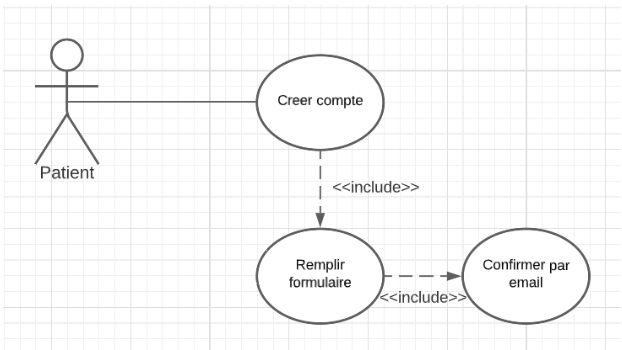
\includegraphics[scale=0.5]{besoins/creer-compte.png}
\end{center}

\subsection{S'authentifier}
\begin{center}
    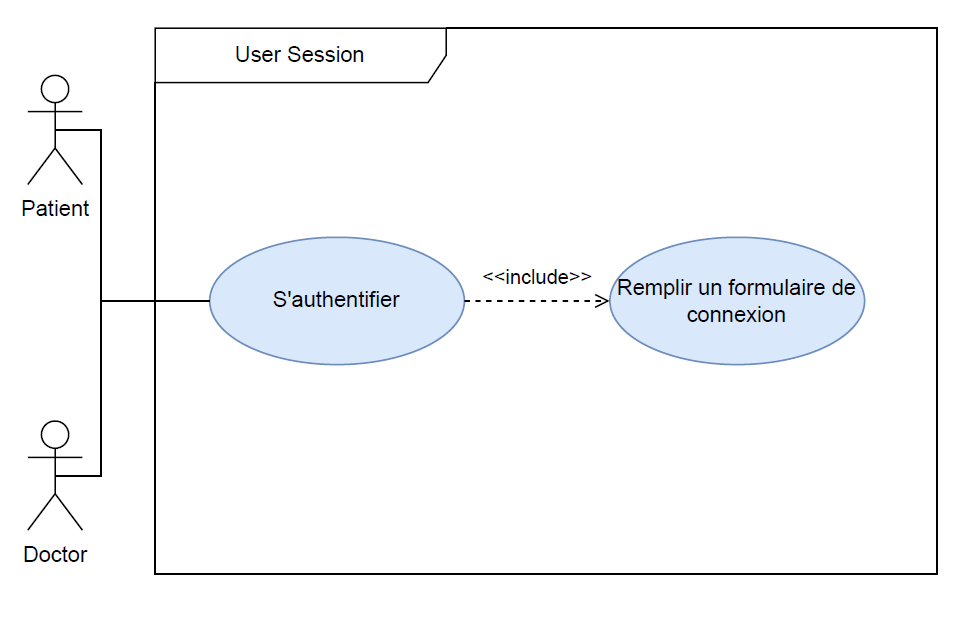
\includegraphics[scale=0.5]{besoins/authentification.png}
\end{center}

\subsection{Gérer les rendez-vous en ligne}
\begin{center}
    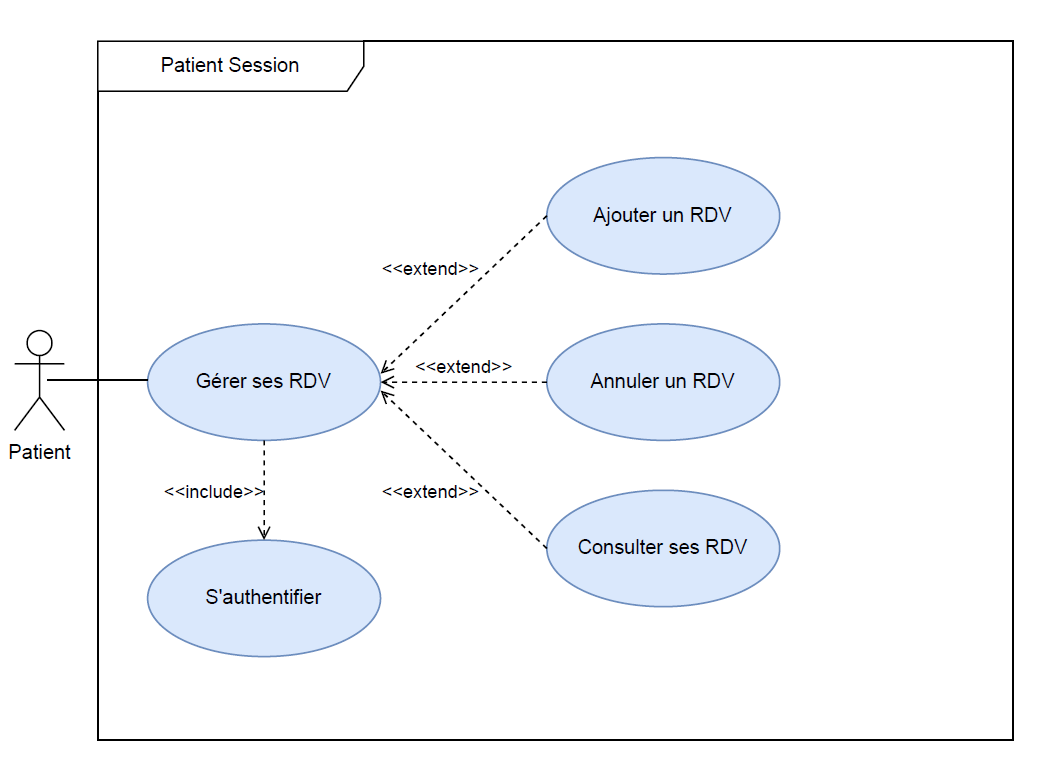
\includegraphics[scale=0.5]{besoins/gerer-rdv-patient.png}
\end{center}

\begin{center}
    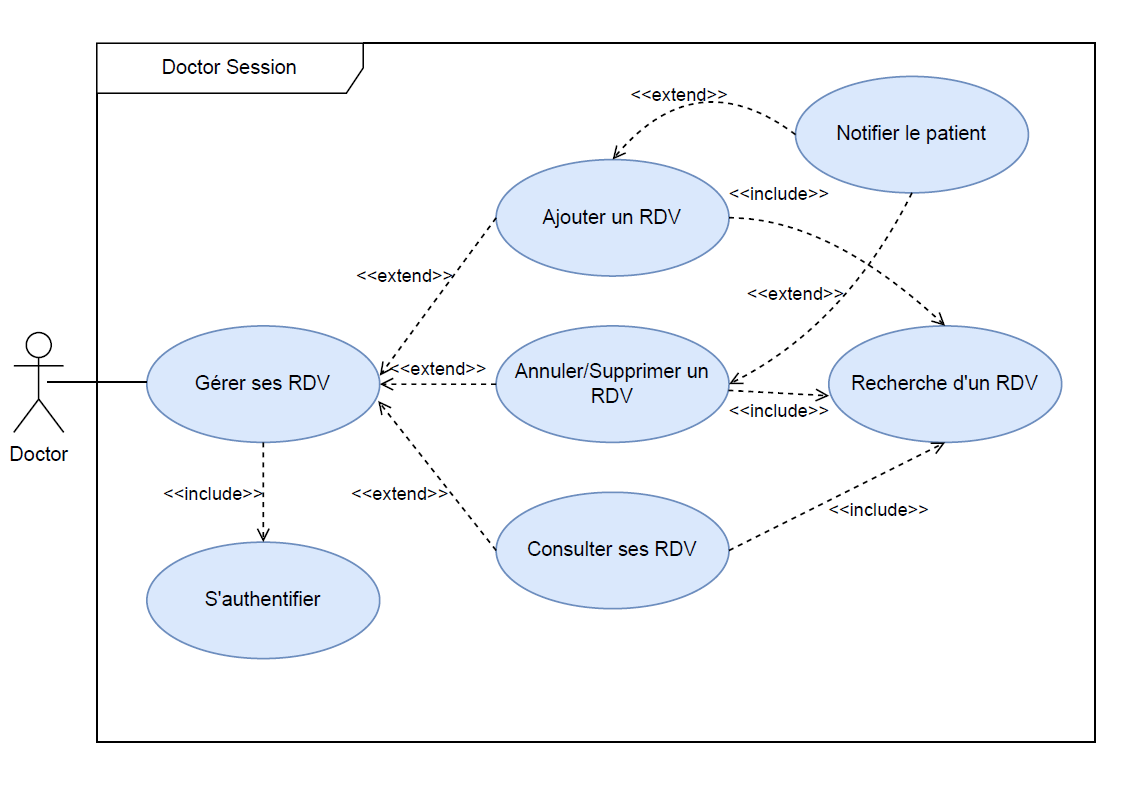
\includegraphics[scale=0.5]{besoins/gerer-rdv-medecin.png}
\end{center}

\subsection{Consulter les rendez-vous}
\begin{center}
    \centering
    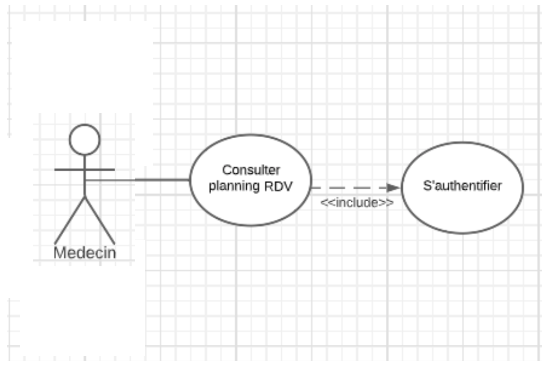
\includegraphics[scale=0.5]{besoins/consulter-rdv.png}
\end{center}

\subsection{Consulter le dossier médical}
\begin{center}
    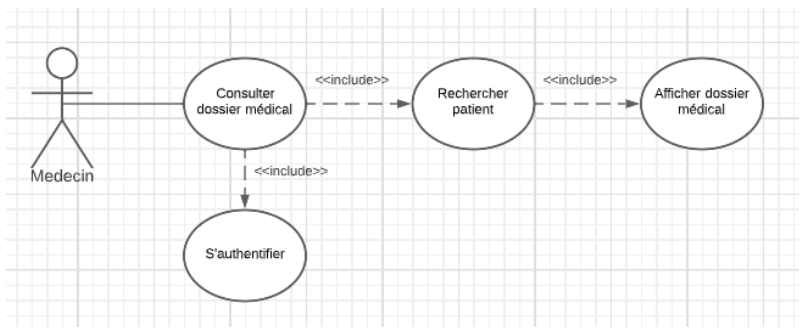
\includegraphics[scale=0.5]{besoins/consulter-dossier-medical.png}
\end{center}

\subsection{Gérer le dossier médical}
\begin{center}
    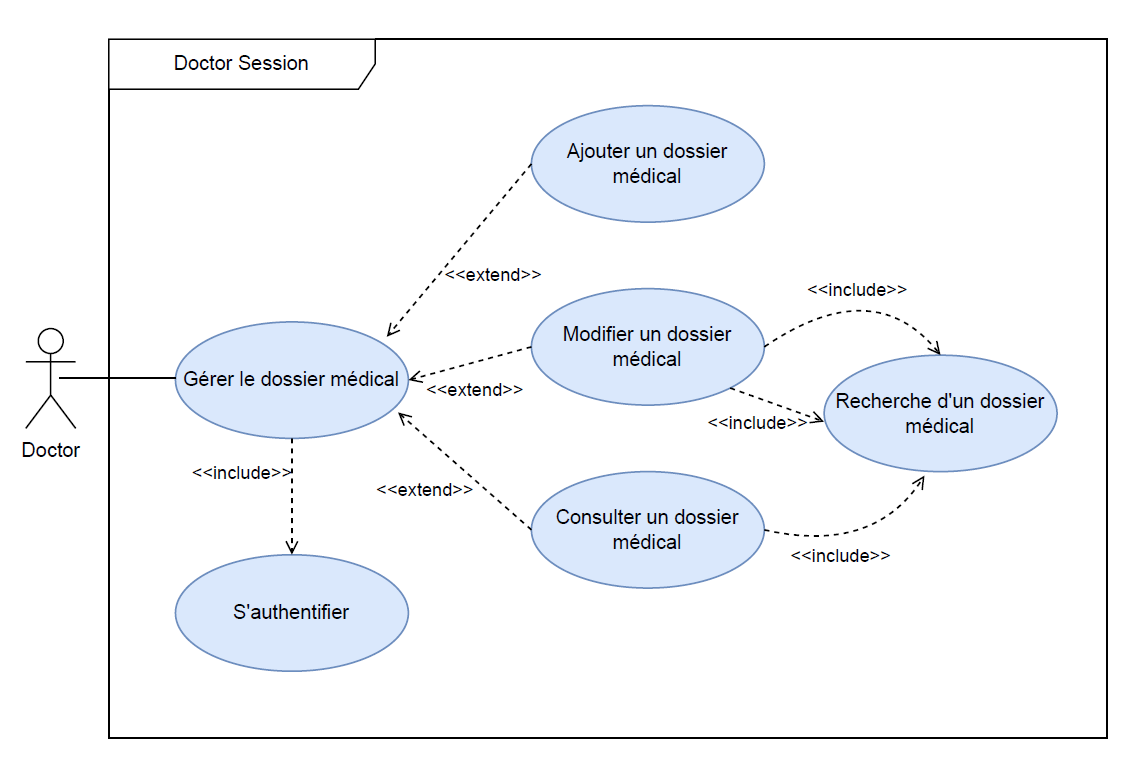
\includegraphics[scale=0.5]{besoins/gerer-dossier-medical.png}
\end{center}

\subsection{Génerer le bilan de santé}
\begin{center}
    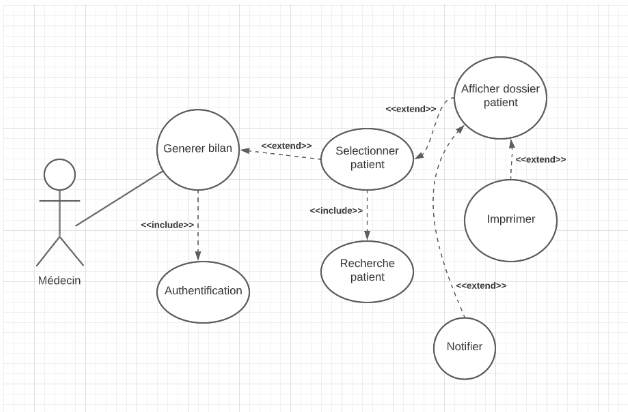
\includegraphics[scale=0.5]{besoins/bilan-sante.png}
\end{center}

\chapter{Conception}


Pour ce projet, nous avons décidé d'utiliser une architecture DDD (Domain-Driven Design) qui se compose de quatre couches distinctes: une couche domaine, 
une couche infrastructure, une couche application et une couche interface utilisateur.
Dans notre application pour le cabinet médical, nous avons adopté une approche DDD pour garantir que notre modèle soit clair et bien structuré. \newline \newline
Dans la couche domaine, on trouve les éléments clés de notre application tels que les patients, les médecins, les rendez-vous, les créneaux horaires, les consultations, 
les adresses des patients et les prescriptions médicales. \newline \newline
Nous avons également mis en place une couche infrastructure en utilisant des bases de 
données relationnelles pour stocker les informations de l'application. Cette couche infrastructure est responsable de créer 
pour chaque classe du domaine une base de données et de gérer les requêtes et les mises à jour dans celles-ci. \newline \newline
Dans la couche interface utilisateur, on a des controllers qui servent d'intérmédiaires entre la partie client et la partie serveur. 
Les controllers reçoivent les entrées utilisateurs, les envoient à la couche application et envoient une réponse au client. \newline \newline
Avec cette architecture DDD, nous avons créé une application structurée pour répondre aux besoins spécifiques d'un cabinet médical. \newline\newline

\chapter{Réalisation}

\section{Outils de développement}

\begin{itemize}
    \item[$\bullet$] \underline{Java} : Nous avons utilisé le langage de programmation orienté objet Java pour notre projet.\newline
    \item[$\bullet$] \underline{ReactJS} : Pour le côté Front-end, nous avons utilisé la bibliothèque JavaScript ReactJS qui est très populaire dans le monde du développement web et 
    très facile d'utilisation. Elle fonctionne avec des composants où chaque composant représente une partie de l'interface utilisateur. Ces composants sont réutilisables ce qui nous permet de gagner du temps. 
    Elle possède également une documentation bien organisée et facile à comprendre. \newline
    \item[$\bullet$] \underline{Maven} : Pour la construction du projet nous avons choisi Maven, un outil de gestion de projet facile à configurer et à utiliser. Il peut être étendu grâce à des plugins pour répondre à des besoins spécifiques. \newline
    \item[$\bullet$] \underline{Git} : Pour pouvoir au mieux travailler sur ce projet chacun de notre côté, nous avons décidé d'utiliser Git qui est un logiciel de gestion de versions décentralisé. Il permet de travailler
    sur des parties différentes du code en même temps et il est très utile pour le travail en équipe.  \newline
    \item[$\bullet$] \underline{Postgresql} : Pour la gestion de nos bases de données nous avons utilisé Postgresql qui est un système de gestion de bases de données relationnelles. Il est fiable et robuste, de plus 
    nous avions déjà utilisé ce système donc c'était facile pour nous de l'utiliser pour notre projet. \newline
    \item[$\bullet$] \underline{JUnit} : Pour les tests, nous avons utilisé JUnit qui est un framework de test unitaire pour Java et qui permet de tester des fragments de code de manière isolée et automatisée.\newline
\end{itemize}


(outils, logiciels, interfaces graphiques, réf biblio)

\chapter{Tests}


\chapter{Résultats}

(Mettre ici les captures et les fonctionnalités)

\chapter{Conclusion}

\end{document}